\title{REPORT}
\author{
        \\
        Department of Electronics And Communication\\
       Model Engineering College\\
       Thrikkakara\\
       \\
       \\\textbf{TEAM MEMBERS}\\
       \\NANDAGOPAN G \\
        VISHNU S MENON     \\
        TEENA M T\\
        DIVYA K\\
        ATHIRA PRAVEEN\\
}
%\date{}

\documentclass[12pt,a4paper,oneside]{report}


\usepackage{amsfonts}
\usepackage{textcomp}
\usepackage{graphicx}
\usepackage{setspace}
\usepackage{fancyhdr}
\usepackage{truncate}
\usepackage{nomencl} 
\usepackage{array}
\usepackage{caption}
\usepackage{subcaption}
\usepackage{subfig}
\usepackage[overload]{textcase}
\renewcommand{\nomname}{List of Abbreviations}
\makenomenclature



\usepackage{titlesec}
\titleformat{\chapter}[display]
  {\normalfont\Large\bfseries\centering}
 {\chaptertitlename\ \thechapter}{20pt}{\LARGE}
\titleformat{\section}{\large\bfseries}{\thesection}{1em}{}
\titleformat{\subsection}{\normalsize\bfseries}{\thesubsection}{1em}{}



\renewcommand{\chaptermark}[1]{\markboth{ \emph{#1}}{}}

\begin{document}
\maketitle
\thispagestyle{empty}

\pagenumbering{roman}



\begin{onehalfspacing}



\pagenumbering{arabic}



\section{INTRODUCTION}



{$\;\;\;\;$}
  
 GSM and GPRS based Designs have developed another innovative and Public utility product for mass communication . This is a Fire Fighting Robot which is used for prevent our houses, offices and shops from Fire.

 The basic idea behind this project is that your robot moves in the suffocated fire area in your houses, offices etc, when you are not at home or office. It will find the existence of fire using IR sensor and when the fire is detected by robot ,it will try to fight with fire using bluer and as well as sent the message to you using SMS or GPRS Packets . Such Devices can be used at different areas of the human life such as offices, houses, factories etc.

Wireless communication has announced its arrival on big stage and the world is going mobile . We want to control everything and without moving an inch. This remote control GSM Fire Fighting Robot is possible through Embedded Systems. The use of “Embedded System in Communication” has given rise to many interesting applications that ensures comfort and safety to human life. 

The main aim of the project will be to design a SMS electronic Fire Fighting Robot toolkit which can replace the traditional Fire Fighting Robot. The toolkit sense the fire and send SMS to owner of the house, The system is made efficient by SIMs so that the SMS can be received by number of device boards in a locality using techniques of time division multiple access.

\newpage
\section{OVERVIEW}
{$\;\;\;\;$}

The main components of the toolkit include microcontroller, GSM modem. These components are integrated with the device board and thus incorporate the wireless features. 
The GSM modem receives the SMS. The AT commands are serially transferred to the modem. In return the modem transmits the stored message through the wireless link. The microcontroller validates the SMS and then perform specific task on the device. The microcontroller used in this case is PIC 16F877A .SIM 300 is used as the GSM modem. The results presented in the thesis support the proper functionalities and working of the system. The timing diagram suggests the response of the modem to various AT (attention) commands.



\section{METHODOLOGY}
{$\;\;\;\;$}
The method used to carry out this project is the principle of serial communication in collaboration with embedded systems.This is a very good project for Industries. 
This project has a GSM Fire Fighting Robot, which will be used as the electronic device, and also a GSM modem, which is the latest technology used for communication between the mobile and the embedded devices.
The basic working process is,when the user wants to receive a SMS on the existence of the fire in their houses or offices, the robot sends a message through the subscriber identity module (SIM) which is inserted in the display system MODEM and fights against the fire.

\newpage
\section{BLOCK DIAGRAM}
{$\;\;\;\;$}



\begin{figure}[h]
\begin{center}
\leavevmode
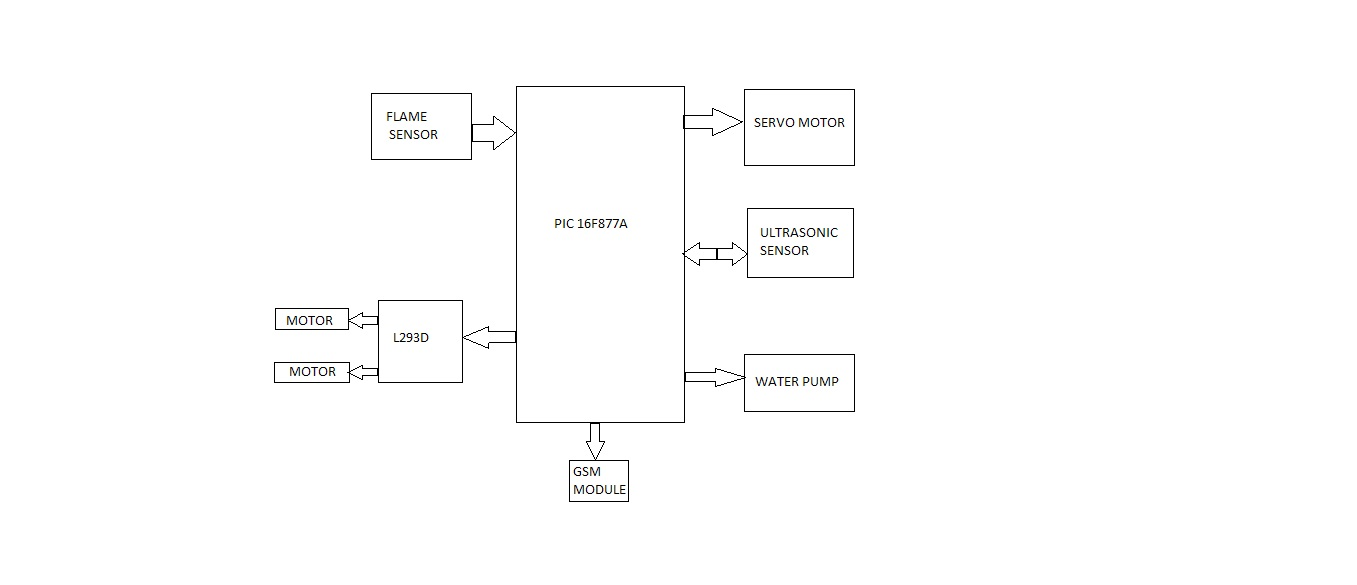
\includegraphics[width=20cm, height=10cm]{blockdiag.jpg}
\end{center}
\label{fig1}
\end{figure}


\newpage
\section{SCOPE OF WORK}
\par
\hspace{.7cm}
  GSM modem (SIM 300) is used as an interface between mobile and microcontroller. It will send message to any phone irrespective of the GSM network through the modem connected to the programmable device.This system can be used to create a safe environment atn a large scale in industries,offices or at places where humans cannot directly enter.\\

\section{USES}
\par
\hspace{.7cm}
Considering the elevated amount of fire accidents leading to the loss of life and property especially due to the lack of timely action, we have come up with a very useful and innovative project. We can use this to secure our houses and offices from fire. 

\section{COMPONENT LIST}
{$\;\;\;\;$}	
\begin{table}[h]
\begin{tabular}{|c|c|c|c|}
\hline
\textbf{COMPONENT} & \textbf{COST(Rs)} & \textbf{QUANTITY} & \textbf{AVAILABILITY}\\
\hline
Fire Sensor module	& 250 & 1 &	Available Online\\
GSM module	& 1100 & 1	& Available\\
PIC 16F877A &	150 & 1 &	Available\\
Motor Driver IC &	55 & 1 &	Available\\
DC Motor &	75 & 2 &	Available\\
Ultrasonic sensor & 950 & 1 & Available\\
Servo Motor & 600 & 1 & Available\\
Comparator IC &	10 & 1	& Available\\
Miscellaneous & 500 & &\\
\hline
\textbf{TOTAL}	& 4000  & &\\
\hline

\end{tabular}
\end{table}

\newpage
\section{CONCLUSION}
\par
\hspace{.7cm}
 GSM and GPRS based Designs have developed another innovative and Public utility product for mass communication .

The project is aimed at developing the security of Home against Intruders, Gas Leak and Fire. 
In any of the above three cases, any one met ,while you are out of your home, thenthe device sends SMS to the emergency no provided to it. The Microcontroller based system continuously watching the security issues of your house, if any mishap condition from above three occurs,it will sense and send a message to your mobile.
					
The main aim of the project will be to design a SMS electronic HOME SECURITY SYSTEM toolkit which can replace the traditional HOME SECURITY SYSTEM. The toolkit send SMS to house owner number, the system is made efficient by SIMs so that the SMS can be received by number of devices boards in a locality using techniques of time division multiple access.

This report demonstrates a brief overview and the feasibility of our project.We are genuinely confident in its feasibility and scope ,as all the components we require are easily available,moreover majority of the concepts involved in this project have been familiarised  through various workshops that we have attended.The TWM workshop on PIC microcontroller and its interfacing,workshop on swarm robotics hosted by roboversity etc. have added to the pre-requisite knowledge that we require for making this project successful.Also,the training that we secured from Bsnl during a brief internship,have familiarised us with the basic concepts of GSM module and its interfacing.

We truly believe in the feasibility and potential of our project,and are confident in its outcome. We hope  that we have succeeded in demonstrating the scope and worth of our project, and we hope that it is kindly acknowledged.\\




\textbf{THANK YOU}
\centering




\end{onehalfspacing}
\end{document}
